\documentclass[11pt,a4paper]{article}

\usepackage[margin=1in]{geometry}
\usepackage{amsmath,amssymb}
\usepackage{booktabs}
\usepackage{array}
\usepackage{tikz}
\usepackage{microtype}
\usepackage[colorlinks=true,linkcolor=black,citecolor=blue,urlcolor=blue]{hyperref}
\usepackage{enumitem}
\usepackage{fancyvrb}
\usepackage{xcolor}

\newcolumntype{L}[1]{>{\raggedright\arraybackslash}p{#1}}

\title{Recursive Self-Improvement via .cgp Cognitive Patches:\\
A Zero-Trust, Verifier-Gated Pipeline for Autonomous LLM Artifact Evolution}
\author{Jean Machuca\\CognitiveOS-Labs \quad ORCID: 0009-0004-9924-2911}
\date{November 2026}

\begin{document}
\maketitle

\begin{abstract}
Recursively training a large language model on its own output is a known
failure amplifier: without external correctness signals, synthetic data
erosion collapses capability and diversity. We present the first specification
and implementation of recursive self-improvement (RSI) as a \emph{distribution
artifact lifecycle} over CognitiveOS \texttt{.cgp} (Cognitive Patch) packages
managed by the Cognitive Package Manager (\texttt{cpm}). Synthetic training
signals are admitted only through an external deterministic verifier
(AST-allowlist plus sandboxed unit-test execution); each generation's LoRA
adapter is fused in FP16 into the master checkpoint (never into quantized
GGUF); promotion of generation $t{+}1$ is decided by an isolated two-benchmark
zero-trust gate with automatic rollback. We release the complete pipeline as
two versioned \texttt{.cgp} artifacts (\texttt{base-model-v0},
\texttt{rsi-controller}), with unit tests, CI packaging, a frozen experimental
protocol (6 cycles, t$=0..5$, three-arm ablation) and a pre-registered
hypothesis set. Empirical multi-generation evidence is pending a GPU training
run and is explicitly \emph{not} claimed here; the separation between what is
measured (pipeline validation) and what is pre-registered (M$_0{\rightarrow}$M$_6$
comparisons) is itself a contribution to reproducible reporting in self-training research.
\end{abstract}

\section{Introduction}

Self-training works when the model's own outputs are filtered by a reliable
signal \cite{zelikman2022star, wang2023selfie, wei2022verifiers}; it fails
catastrophically without one \cite{shumailov2024nature}. CognitiveOS
distributes models and skills as \texttt{.cgp} archives with an
install-time lifecycle (\texttt{cpm}) that includes integrity verification,
hardware audits, and (via the Controller Pattern) on-device fine-tuning with
rollback semantics. This raises a natural question: can the artifact itself
carry the \emph{entire} self-improvement lifecycle --- generation,
verification, tuning, merging, quantization, benchmark gating, promotion and
rollback --- as auditable, versioned content?

We answer affirmatively at the engineering level and pre-register the
empirical claim. Our three enforced invariants --- an FP16/BF16 master
precision policy, a deterministic-verification admission policy, and a
zero-trust promotion policy --- are enforced in code, not by convention.

\subsection{Contributions}
\begin{enumerate}[leftmargin=1.6em]
  \item A \texttt{.cgp}-native RSI architecture with three enforced invariants
        (Sections~\ref{sec:arch}--\ref{sec:gate}).
  \item \texttt{rsi-controller.cgp}: a working MCP stdio controller implementing
        the verifier, the promotion gate, the \texttt{cpm tune} Controller
        Pattern, and pipeline status reporting (Section~\ref{sec:impl}).
  \item A frozen, executable protocol (6 cycles; arms A/B/C; isolated
        benchmarks; fixed seeds; verbatim JSONL logging)
        (Section~\ref{sec:protocol}).
  \item An honest validation ledger and a failure/safety analysis with
        pre-registered falsifiers (Sections~\ref{sec:validation}--\ref{sec:limits}).
\end{enumerate}

\section{Background and related work}

\paragraph{Low-rank adaptation.} LoRA \cite{hu2022lora} constrains weight
updates to low-rank matrices, making per-generation fine-tuning cheap enough
to repeat recursively; QLoRA \cite{dettmers2023qlora} shows 4-bit inference
over frozen weights with adapter training, but we deliberately avoid
backpropagating through quantized checkpoints --- our master is never
quantized between merges.

\paragraph{Self-improvement and self-training.} STaR \cite{zelikman2022star}
and Self-Instruct \cite{wang2023selfie} bootstrap reasoning from the model's
own outputs; both rely on filtering (rationales \emph{validated} by outcome,
or task diversity heuristics). Verifier-trained math reasoning
\cite{wei2022verifiers} shows outcome-based checking outperforms reward-model
pseudo-labels --- our verifier is the same idea lifted to an artifact-level
gate.

\paragraph{Model collapse.} Shumailov et al. \cite{shumailov2024nature}
demonstrate that unfiltered recursive self-consumption erodes tails of the
data distribution. Our admission control (100\% deterministic verification +
20\% fixed anchor replay) is a direct countermeasure, and arm C of our
ablation measures its necessity.

\paragraph{Instruction tuning.} Ouyang et al. \cite{ouyang2022instructgpt}
anchor our general-capability regression benchmark conceptually.

\paragraph{CognitiveOS \texttt{.cgp} format.} \texttt{.cgp} archives bundle a
manifest (\texttt{cognitive.json}), prompts, MCP tools, and/or weights;
\texttt{cpm pack}/\texttt{verify} enforce archive integrity and manifest
schema (V001--V012). A base-model package can declare a \texttt{training}
block read by \texttt{cpm tune}; the designated MCP tool then performs
fine-tuning and the artifact is promoted or rolled back at the package
boundary.

\section{System architecture}\label{sec:arch}

\begin{figure}[ht]
\centering
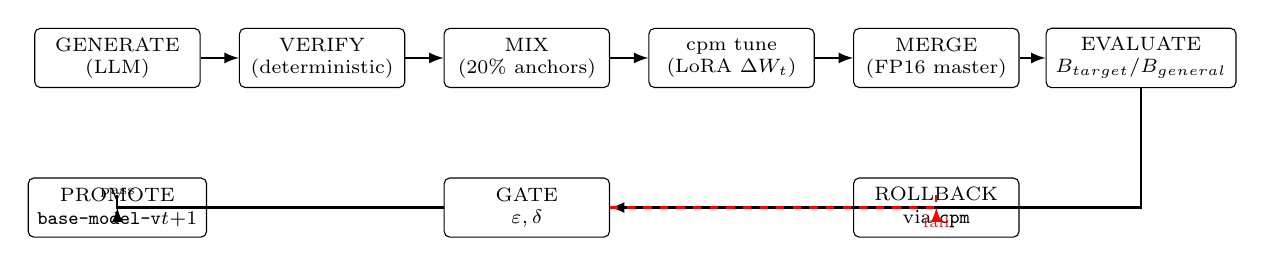
\begin{tikzpicture}[
  stage/.style={draw, rounded corners=2pt, align=center, minimum height=7.5mm,
                minimum width=21mm, font=\scriptsize},
  ok/.style={-latex, thick},
  bad/.style={-latex, thick, dashed, red}
]
\node[stage] (gen) at (0,0) {GENERATE\\ (LLM)};
\node[stage] (ver) at (2.6,0) {VERIFY\\ (deterministic)};
\node[stage] (mix) at (5.2,0) {MIX\\ (20\% anchors)};
\node[stage] (tune) at (7.8,0) {cpm tune\\ (LoRA $\Delta W_t$)};
\node[stage] (merge) at (10.4,0) {MERGE\\ (FP16 master)};
\node[stage] (eval) at (13,0) {EVALUATE\\ $B_{target} / B_{general}$};
\node[stage] (gate) at (5.2,-1.9) {GATE\\ $\varepsilon, \delta$};
\node[stage] (promote) at (0,-1.9) {PROMOTE\\ \texttt{base-model-v}$t{+}1$};
\node[stage] (rollback) at (10.4,-1.9) {ROLLBACK\\ via \texttt{cpm}};

\draw[ok] (gen) -- (ver);
\draw[ok] (ver) -- (mix);
\draw[ok] (mix) -- (tune);
\draw[ok] (tune) -- (merge);
\draw[ok] (merge) -- (eval);
\draw[ok] (eval) |- (gate);
\draw[ok] (gate) -| (promote) node[midway, above, font=\tiny] {pass};
\draw[bad] (gate) -| (rollback) node[midway, below, font=\tiny] {fail};
\end{tikzpicture}
\caption{One RSI cycle. Unverified samples never reach \texttt{cpm tune};
promotion is the only path to replacing $M_t$, and it is gated by isolated
benchmarks with automatic rollback on failure.}
\label{fig:loop}
\end{figure}

\subsection{Precision-preserving weight pipeline}\label{sec:precision}

The master at every generation $t$ is FP16/BF16 \texttt{.safetensors}. The
adapter $\Delta W_t$ is trained on $M_t^{\mathrm{FP16}}$ and fused in FP16
via \texttt{merge\_and\_unload()}; only the fused master
$M_{t+1}^{\mathrm{FP16}}$ is quantized
(Q8\_0/Q6\_K) to the deployable GGUF artifact packaged as
\texttt{base-model-v{t+1}.cgp}. LoRA is never merged into quantized weights:
quantization error would compound across generations and the promotion gate
would silently compare noise against improvements. The merger asserts that
every tensor in the fused artifact is F16/BF16 before returning.

\subsection{Self-generated data with deterministic verification}\label{sec:verify}

Domain: Python algorithmic synthesis --- correctness is execution-checkable.
Each generation:
\begin{enumerate}[leftmargin=1.6em]
  \item The model synthesizes a candidate problem with hidden tests (JSON).
  \item The model solves it.
  \item The \textbf{external verifier} decides admission: (a) AST allowlist
        (\texttt{math}, \texttt{collections}, \texttt{itertools},
        \texttt{functools}, \texttt{heapq}, \texttt{bisect}, \texttt{string},
        \texttt{re}, \texttt{operator}, \texttt{typing},
        \texttt{dataclasses}); (b) no \texttt{eval}, \texttt{exec},
        \texttt{open}, \texttt{\_\_import\_\_}, \texttt{input},
        \texttt{compile}; no dunder attribute access; (c) sandboxed
        subprocess (\texttt{RLIMIT\_CPU=5}, \texttt{RLIMIT\_AS=256\,MiB},
        \texttt{RLIMIT\_NPROC=64}, \texttt{RLIMIT\_FSIZE=1\,MiB}, 6\,s
        wall clock); (d) the hidden suite must pass completely.
  \item Verified samples are mixed with a fixed 20\% anchor replay buffer
        (16 verifier-passing problems, seeded sampling).
\end{enumerate}

Unverified outputs are discarded; there is no override. An LLM-as-judge is
deliberately absent from the verdict path.

\subsection{Zero-trust promotion gate}\label{sec:gate}

\begin{equation}
\mathrm{promote} \iff
s(M_{t+1}, B_{\mathrm{target}}) > s(M_t, B_{\mathrm{target}}) + \varepsilon
\;\land\;
s(M_{t+1}, B_{\mathrm{general}}) \ge s(M_t, B_{\mathrm{general}}) - \delta
\label{eq:gate}
\end{equation}

with $\varepsilon = 0.02$, $\delta = 0.01$; strict-greater semantics
implemented as $a - b > \varepsilon \land \lnot\mathrm{isclose}(a-b,
\varepsilon, 10^{-9})$ to defeat floating-point leakage. On failure:
rollback via \texttt{cpm install}, failure-mode logging, and bounded
hyperparameter adjustment (target-miss $\Rightarrow$ lr/2; general-regression
$\Rightarrow$ lr/2 and data-temperature/2; both $\Rightarrow$ lr/2 and
rank/2, floor 4), one retry, then the arm stops.

\subsection{Benchmarks and isolation}

$B_{\mathrm{target}}$: 8 held-out algorithmic problems (fib, vowel counting,
second-largest, gcd, Roman numerals, longest run, clean-palindrome,
sum-of-squares-of-evens), verified solvable through the same verifier (8/8).
$B_{\mathrm{general}}$: 8 instruction-following items (closed-vocabulary
answers). Neither is visible to synthesis, verification training mixes, or
the tuner; $B_{\mathrm{target}}$ feeds only the gate.

\subsection{\texttt{.cgp} packaging (Controller Pattern)}\label{sec:impl}

\texttt{base-model-v0.cgp} (805\,B): \texttt{wide\_model} manifest, remote FP16
safetensors (HF \texttt{google/gemma-3-1b-it}); declares a
\texttt{brain.training} block (rank 16, $\alpha$ 32, 2 epochs, lr $2\times
10^{-4}$, min\_samples 50). \texttt{rsi-controller.cgp} (5.5\,kB): MCP stdio
server exposing \texttt{cognitiveos.rsi.verify} (the deterministic verifier),
\texttt{cognitiveos.rsi.gate} (the gate of Eq.~\ref{eq:gate}),
\texttt{cognitiveos.rsi.tune} (fail-closed without a GPU stack),
\texttt{cognitiveos.rsi.status} (metrics summary). Both archives pass
\texttt{cpm pack} and \texttt{cpm verify} (v1.0.9-alpha).

\paragraph{Spec/implementation divergence (documented).}
\texttt{brain.training} is read by \texttt{cpm tune} but is absent from both
schemas (accepted via unknown-property tolerance); the \texttt{dependencies}
manifest field is rejected by cpm's validator (V006);
\texttt{brain.wide\_model.routing} shapes diverge between spec and
implementation --- omitted. Full
notes in the code repository (\texttt{docs/cpm-implementation-notes.md}).

\section{Experimental protocol (frozen)}\label{sec:protocol}

\textbf{Claim under test.} A \texttt{.cgp}-packaged LLM can recursively
self-improve on a verifiable domain across N$\ge$5 (here 6, t$=0..5$)
generations without collapse, retaining general capability within $\delta$.

\textbf{Pre-registered hypotheses.} H5: gate-promoted final model M$_6$ beats
M$_0$ by $\ge$5 points on $B_{\mathrm{target}}$ with B$_{general}$ retention
$\ge -\delta$. H6a: arm C (verifier bypassed) regresses or collapses vs arm A.
H6b: arm B (single-shot LoRA, M$_0$-data-only, equal total rank-steps)
underperforms arm A. H7: per-generation FP16$\rightarrow$Q8\_0 drift
$<$ 1 point B$_{\mathrm{target}}$, top-1 agreement $\ge$99\%. All hypotheses
are falsifiable; rejection will be reported as such.

\textbf{Arms.} A: full recursive loop. B: single LoRA over M$_0$ with equal
total compute on M$_0$-generated verified data. C: as A, verifier verdicts
ignored (all samples admitted), gate unchanged. All arms share benchmarks,
seeds (1337 primary; 2026/42 for error bars), anchors, budget.

\textbf{Metrics per generation.} synthetic pass rate; train loss; adapter
norm $\lVert\Delta W_t\rVert$; B$_{\mathrm{target}}$/B$_{\mathrm{general}}$
scores; gate decision; inference latency. Logged verbatim to
\texttt{runs/metrics.jsonl}; ablation logs under \texttt{runs/ablation-*}.

\textbf{Execution.} GPU host: 1$\times$24\,GB GPU, \texttt{cpm},
\texttt{code-inference} or vLLM serving FP16 weights, $\ge$200\,GB disk.
Runbook: code repo \texttt{docs/REPRODUCIBILITY.md}.

\section{Pipeline validation (executed 2026-11-17)}\label{sec:validation}

All rows re-verifiable; none are capability measurements.

\begin{table}[ht]
\centering
\small
\begin{tabular}{L{6.6cm} L{6.2cm}}
\toprule
\textbf{Check} & \textbf{Result} \\
\midrule
Unit tests (verifier, gate, replay, controller, metrics) & 20/20 pass \\
Mock e2e, happy path (2 gen) & 2/2 promoted; metrics JSONL well-formed \\
Mock e2e, rejection path & gen 1 rejected; rollback invoked; failure logged \\
Anchor replay set & 16/16 pass the deterministic verifier \\
Benchmark solvability & 8/8 reference solutions pass the verifier \\
\texttt{cpm pack}/\texttt{cpm verify} & both \texttt{.cgp} archives valid \\
Float-noise $\varepsilon$ semantics & strict gate preserved (\texttt{isclose}) \\
\bottomrule
\end{tabular}
\caption{Executed checks at the time of writing.}
\label{tab:measured}
\end{table}

\section{Empirical status and pre-registered comparison}\label{sec:pending}

\textbf{No M$_0{\rightarrow}$M$_6$ capability numbers exist yet.} The table
placeholder below is pre-registered and will be filled exclusively from
\texttt{runs/metrics.jsonl} after the GPU run.

\begin{table}[ht]
\centering
\small
\begin{tabular}{c c c c c c c c c}
\toprule
gen & pass\% & loss & $\lVert\Delta W\rVert$ & B$_t$ & $\Delta$B$_t$ & B$_g$ & $\Delta$B$_g$ & verdict \\
\midrule
0 (M$_0$) & -- & -- & -- & TBD & -- & TBD & -- & baseline \\
1--6 & TBD & TBD & TBD & TBD & TBD & TBD & TBD & TBD \\
\bottomrule
\end{tabular}
\caption{Pre-registered results table (to be filled verbatim from logs).}
\label{tab:pending}
\end{table}

\section{Failure and safety analysis}\label{sec:failure}

\begin{table}[ht]
\centering
\small
\begin{tabular}{L{0.9cm} L{4.6cm} L{6.6cm}}
\toprule
\# & \textbf{Failure} & \textbf{Response (implemented)} \\
\midrule
F1 & B$_{\mathrm{target}}$ gain $\le \varepsilon$ & rollback; lr/2; retry once, else stop arm \\
F2 & B$_{\mathrm{general}}$ regression $> \delta$ & rollback; lr/2 + T/2; retry once, else stop \\
F3 & Both gates fail & rollback; lr/2 + rank/2 (floor 4); one retry, else stop \\
F4 & Malicious/invalid synthetic sample & AST/sandbox/tests reject (fail closed) \\
F5 & Verifier timeout/crash & sample discarded; pass-rate drops; no admission \\
F6 & Divegent training (NaN) & gate cannot pass; rollback via F1--F3 \\
F7 & Quantization drift & top-1/KL measurement required per export; fail export otherwise \\
F8 & Catastrophic forgetting & anchor coverage checked; B$_{\mathrm{general}}$ regression bound $\delta$ \\
F9 & Endpoint unreachable & generation skipped; pass rate 0 $\Rightarrow$ no promotion \\
F10 & Rollback failure & fail loudly; promotion never occurred \\
\bottomrule
\end{tabular}
\caption{Failure taxonomy and implemented responses.}
\label{tab:failures}
\end{table}

Quantization drift (F7) is measured, not assumed: per merge, top-1 agreement
and mean KL between the FP16 master and its Q8\_0 export are recorded on 64
fixed $B_{\mathrm{target}}$ prompts; acceptance requires $\ge$99\% agreement
and B$_t$(GGUF) within 0.5 points of B$_t$(FP16).

\section{Limitations}\label{sec:limits}

(i)~Empirical gap --- the M$_0{\rightarrow}$M$_6$ evidence is pending the
GPU run; no capability claim is made. (ii)~Single domain (Python algorithmic
synthesis) and single base (gemma-3-1b-it). (iii)~Benchmark size (8/8) makes
absolute deltas noisy; report $n$ and CIs. (iv)~Test-suite-as-spec bounds
correctness claims to the suite. (v)~GPU non-determinism requires multi-seed
reporting for headline numbers (protocol registries seeds). (vi)~The verifier
allowlist may reject correct exotic solutions; rejection rate is logged.

\section{Conclusion}

The \texttt{.cgp} format carries a complete, auditable self-improvement
lifecycle: verify, tune, merge, quantize, gate, promote, roll back. What
exists today is the machinery, packaged and tested; what remains is a
GPU-hours experiment, precisely specified and pre-registered. We decline to
claim empirical wins we have not measured, and we ship the shortest path to
measuring them.

\bibliographystyle{unsrt}
\bibliography{references}

\end{document}
